%!xelatex = 'xelatex --halt-on-error %O %S'

\documentclass{thuemp}
\begin{document}

% 标题,作者
\emptitle{光栅衍射实验报告}
\empauthor{江灿}{2019011325}

% 奇数页页眉 % 请在这里写出第一作者以及论文题目
\fancyhead[CO]{{\footnotesize 江灿: 光栅衍射实验报告}}


%%%%%%%%%%%%%%%%%%%%%%%%%%%%%%%%%%%%%%%%%%%%%%%%%%%%%%%%%%%%%%%%
% 关键词 摘要 首页脚注
%%%%%%%%关键词
\Keyword{光栅衍射,波长,光栅常数,最小偏向角}
\twocolumn[
\begin{@twocolumnfalse}
\maketitle

%%%%%%%%摘要
\begin{empAbstract}
	本次实验是光栅衍射实验,进一步熟悉了分光计的调整与使用,
	利用衍射光测定了四种光波的波长与光栅常数,并与标准值进行对比。
	最后使用最小偏向角法测出波长较长的黄线的波长
\end{empAbstract}
\empfirstfoot{2022-04-03}{软件02}{双日下M}{7号}
%%%%%%%%首页角注,依次为实验时间、报告时间、学号、email
\end{@twocolumnfalse}
]
%%%%%%%%!首页角注可能与正文重叠,请通过调整正文中第一页的\enlargethispage{-3.3cm}位置手动校准正文底部位置:
%%%%%%%%%%%%%%%%%%%%%%%%%%%%%%%%%%%%%%%%%%%%%%%%%%%%%%%%%%%%%%%%
%  正文由此开始
\wuhao 
%  分栏开始

\section{实~~验~~目~~的}
略

%%%%%%%%%%%%%%%%%%%%%%%%%%%%%%%%%%%%%%%%%%%%%%%%%%%%%%%%%%%%%%%%
\section{实~~验~~仪~~器}
略
\section{实~~验~~原~~理}
略
%%%
\section{实~~验~~步~~骤} 
略
%%%%%%%%%%%%%%%%%%%%%%%%%%%%%%%%%%%%%%%%%%%%%%%%%%%%%%%%%%%%%%%%
%%%%%%%%%%%%%%%%%%%%%%%%%%%%%%%%%%%%%%%%%%%%%%%%%%%%%%%%%%%%%%%%
\newpage 
\section{实~~验~~数~~据}

\subsection{实~~验~~数~~据~~整~~理}
入射角 i = 0°时,测定光栅常数和光波波长的数据整理如下\\
其中入射角方位$\varphi _{10} = 252°41' \ \varphi _{20} = 72°41'$
\begin{figure}[H]
	\centering
	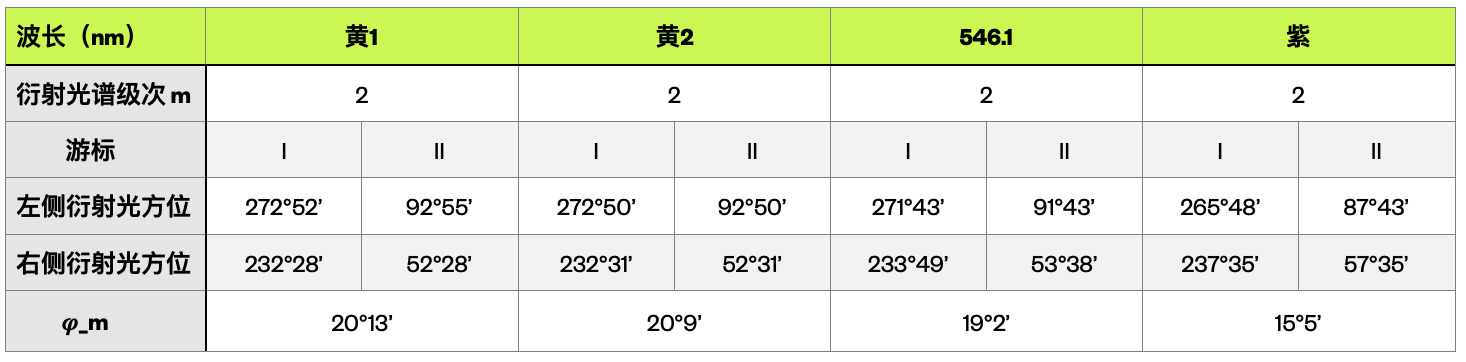
\includegraphics[width=0.8\linewidth]{./image/1.png}
	\caption{测定光栅常数和光波波长数据} 
	\label{png:1}
\end{figure}
入射角 $i = 15°0'$时,测量波长较短的黄线的波长的数据整理如下\\
其中光栅平面法线方位$\varphi _{1n} = 252°41'\ \varphi _{2n} = 72°41'$
\begin{figure}[H]
	\centering
	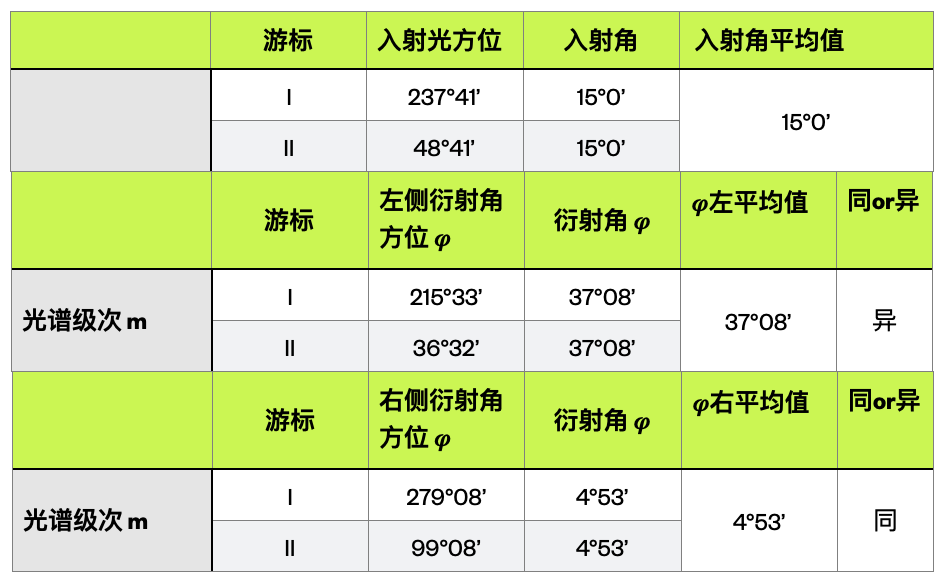
\includegraphics[width=0.8\linewidth]{./image/2.png}
	\caption{测量波长较短的黄线的波长} 
	\label{png:2}
\end{figure}
\newpage
\subsection{数~~据~~处~~理}
相对误差计算为
$$\frac{\delta}{\mu}=\frac{|x-\mu|}{\mu}\times 100\%$$
其中x为测量值,$\mu$为标准值
\subsubsection{级次的处理}
在课前预习题中已经计算出了$$(\frac{\Delta d}{d})^2=(\frac{\Delta \varphi _m}{tan\varphi })^2$$
$$(\frac{\Delta \lambda}{\lambda})^2=(\frac{\Delta d }{d})^2+(\frac{1}{tan \varphi _m})^2\Delta\varphi _m^2+(\frac{\Delta m}{m})^2$$
在实际测量时,应该在能看清的基础上,尽可能的选择级次更大的进行测量,减少偏差。\\
因此在第一个实验中,选择了测量级次m=2进行实验测量
\subsubsection{光栅常数和光波波长}
\subsubsection*{d的求解:}
已经测出$\varphi _m = 19°2'$\\可求出$\Delta \varphi _m = \frac{\sqrt{2}}{2}=0.707'$
$$ d = \frac{m \lambda }{sin \varphi _m}=3349.1nm$$
$$\Delta d=\lambda\sqrt{(\frac{\Delta d }{d})^2+(\frac{1}{tan \varphi _m})^2\Delta\varphi _m^2+(\frac{\Delta m}{m})^2}=2.2nm$$
求得$d=(3349.1\pm2.2nm)$
\subsubsection*{$\lambda$的求解:}
$$d sin\varphi _m = m\lambda$$
$$\lambda = \frac{d sin\varphi _m}{m} $$
\begin{enumerate}
	\item 黄光1($\varphi _m=20°13'$)
	$$\lambda = \frac{d sin\varphi _m}{m} =578.6nm \quad \Delta \lambda = 0.3 nm$$
	$$\lambda = (578.6\pm0.3) nm)$$
	$$\frac{\delta}{\mu}=\frac{|578.6-579.1|}{579.1}\times 100\%= 0.01\%$$

	\item 黄光2($\varphi _m=20°9'$)
	$$\lambda = \frac{d sin\varphi _m}{m} =576.8nm \quad \Delta \lambda = 0.4 nm$$
	$$\lambda = (576.8\pm0.4) nm)$$
	$$\frac{\delta}{\mu}=\frac{|576.8-577.0|}{577.0}\times 100\%= 0.01\%$$

	\item 紫光($\varphi _m=15°5'$)
	$$\lambda = \frac{d sin\varphi _m}{m} =435.7nm \quad \Delta \lambda = 0.4 nm$$
	$$\lambda = (435.7\pm0.4) nm)$$
	$$\frac{\delta}{\mu}=\frac{|435.7-435.8|}{435.8}\times 100\%= 0.01\%$$

\end{enumerate}
\subsubsection{波长较短的黄线的波长}
$$d(sin \varphi  +sin i )=m\lambda,i=15°,m=2$$可求得\\
$\varphi _{m左}=37°08'$ \ 异侧$\lambda=576.9nm$\\
$\varphi _{m右}=4°53'$\quad 同侧$\lambda=576.2nm$\\
$$\bar{\lambda}=\frac{\lambda_1+\lambda_2}{2}=576.6nm$$
相对误差为:
$$\frac{\delta}{\mu}=\frac{|576.6-577.0|}{577.0}\times 100\% = 0.09\%$$

\subsubsection{最小偏向角测较长黄光波长}
$$2 d \sin \frac{\delta}{2} = m\lambda , m=0,\pm1,\pm2,\pm3,···$$
测量出$2\delta = 40°6'$即$\delta = 20°3'$,此时级次m=2,带入可求得$\lambda = 579.4$
\\相对误差为:
$$\frac{\delta}{\mu}=\frac{|579.4-579.1|}{579.1}\times 100\%= 0.06\%$$与实际值误差较小。
%%%%%%%%%%%%%%%%%%%%%%%%%%%%%%%%%%%%%%%%%%%%%%%%%%%%%%%%%%%%%%%%
\section{实~~验~~总~~结}
这次实验延续着上次分光计的时间,
需要在开始调节望远镜,
平行光管,
使得二者的光轴都垂直于分光计主轴。
这个环节在上一次实验的时候很艰难,不过在这次实验时,遵循着先粗调后细调,
调节的过程比上次轻松了不少。

不过在三棱镜调好之后,换上光栅的时候却一直无法找到像,最后感谢助教的帮助成功的完成调节。

最后在测量最小偏向角的时候,刚开始直接测的$\delta$,后来为提高测量精度,重新测量了$2\delta$。

这是第二次的光学实验,感受和上次相似,光学实验对于眼睛的考验是很大的,同时也感谢助教的耐心指导,使得这次实验顺利完成
%%%%%%%%%%%%%%%%%%%%%%%%%%%%%%%%%%%%%%%%%%%%%%%%%%%%%%%%%%%%%%%%
\section*{原~~始~~数~~据}
后附页
\newpage





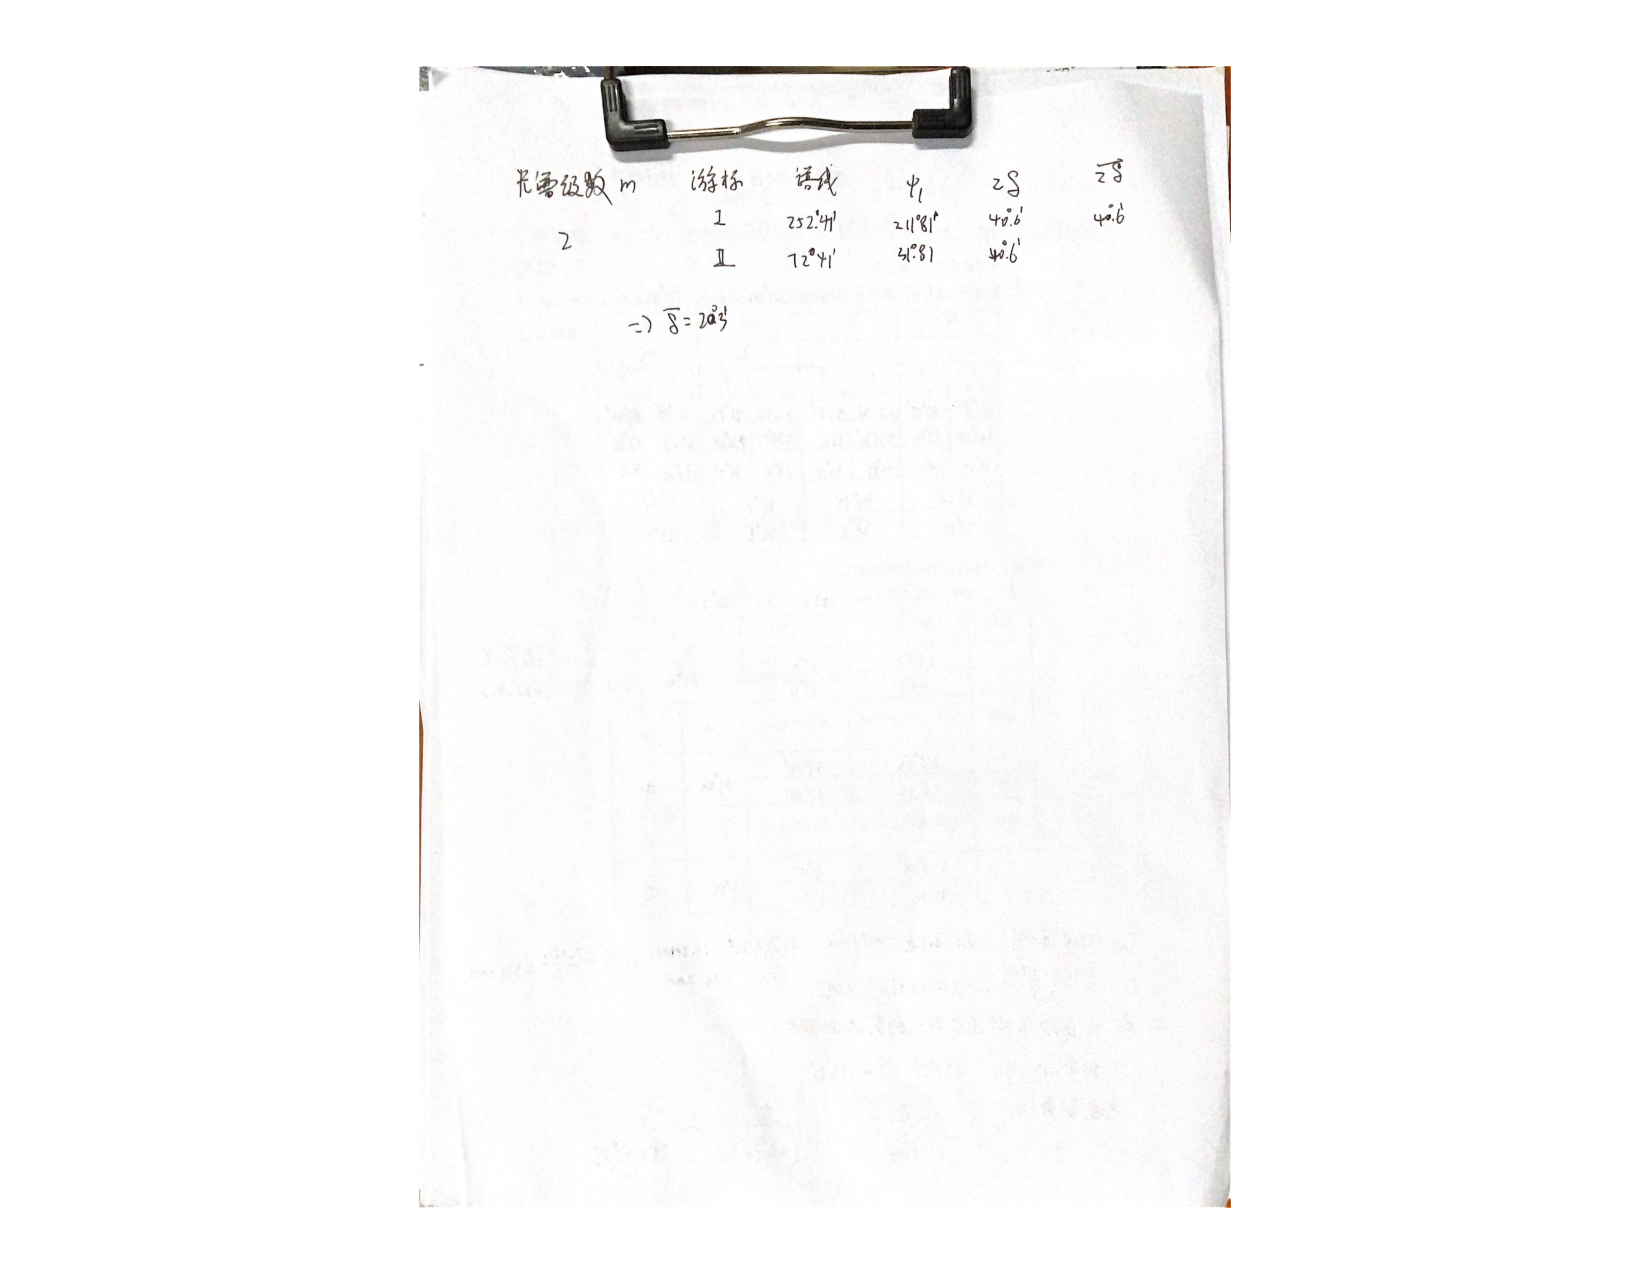
\includepdf[pages=-]{./image/1.pdf}













\newpage
%%%%%%%%%%%%%%%%%%%%%%%%%%%%%%%%%%%%%%%%%%%%%%%%%%
%  参考文献
%%%%%%%%%%%%%%%%%%%%%%%%%%%%%%%%%%%%%%%%%%%%%%%%%%%%%%%%%%%%%%%%
%  参考文献按GB/T 7714-2015《文后参考文献著录规则》的要求著录. 
%  参考文献在正文中的引用方法:\cite{bib文件条目的第一行}

\renewcommand\refname{\heiti\wuhao\centerline{参考文献}\global\def\refname{参考文献}}
\vskip 12pt

\let\OLDthebibliography\thebibliography
\renewcommand\thebibliography[1]{
  \OLDthebibliography{#1}
  \setlength{\parskip}{0pt}
  \setlength{\itemsep}{0pt plus 0.3ex}
}

{
\renewcommand{\baselinestretch}{0.9}
\liuhao
\bibliographystyle{gbt7714-numerical}
\bibliography{./TempExample}
}


\end{document}
